%% ============================================================
%%  STANDARD PREAMBLE (article, lecture notes)
%% ============================================================

% ---------- Document class and page layout ----------
\documentclass[11pt]{article}      % Basic document type, 11pt body text
\usepackage[margin=1in]{geometry}  % Sets page margins to 1 inch on all sides

% ---------- Paragraph style ----------
\usepackage{setspace}              % Lets you set the line spacing of the whole document
\setstretch{1.2}                   % Line spacing factor: 1.0 = single (default), 1.2 = slightly airy, 1.5 = very loose
\setlength{\parindent}{2em}        % First-line indent of each paragraph
\setlength{\parskip}{1\baselineskip} % Extra vertical gap between paragraphs

% ---------- Math ----------
\usepackage{amsmath,amssymb}       % Core math: align, cases, \text{}, \boxed{}, plus extra symbols (\mathbb, \hbar, ...)

% ---------- Colors and boxes ----------
\usepackage{xcolor}                % Lets you use colors (\textcolor{red}{...})
\usepackage{mdframed}              % Boxes around text that can break across pages (theorems, key results)

% ---------- Diagrams ----------
\usepackage{tikz-cd}               % Commutative diagrams / arrow diagrams (also loads tikz)
\usepackage{tikz}                  % General-purpose drawing: lines, shapes, plots
\usetikzlibrary{arrows.meta, positioning} % arrows.meta: more arrow tip styles; positioning: place nodes "right=of A"

% ---------- Text layout ----------
\usepackage{multicol}              % Multi-column text (\begin{multicols}{2} ... \end{multicols})
\usepackage{indentfirst}           % Indents the first paragraph after a heading (article class skips it by default)

% ---------- Hyperlinks (load last) ----------
\usepackage[hidelinks]{hyperref}   % Clickable TOC, \ref, \eqref, \cite; hidelinks = no colored text or boxes

% ---------- Equation numbering ----------
\numberwithin{equation}{section}   % Equation counter resets in each section
\renewcommand{\theequation}{\thesection.\arabic{equation}} % Displays numbers as section.equation, e.g. (2.3)

% ---------- Title block ----------
\title{Advanced Material Physics}
\author{Duy M. Dao}
\date{\today}                      % Compile date; replace with a fixed date if you prefer

\begin{document}
\maketitle                         % Prints title, author, date
%\tableofcontents                   % Clickable table of contents

\newpage

\part{Dielectric Polarization under Static Electric Field}

\paragraph{Unit system used in this note.}
\textcolor{red}{Throughout this note, the unit system is chosen such that $4\pi\epsilon_0 = 1$.}

\section{Multipole Expansion of a Point Cloud}

\paragraph{Potential of a point cloud and the need for an expansion.}
Consider $N$ point charges $q_i$ at positions $\vec r_i$, which together form a \textcolor{blue}{point cloud}. The electric potential at $\vec R$ is the sum of the contributions of all point charges,
\begin{equation*}
    \phi(\vec R) = \sum_{i=1}^{N} \frac{q_i}{|\vec R - \vec r_i|}.
\end{equation*}
In general, this potential depends on the charge positions in a complicated way. Far from the cloud, however, the \textcolor{blue}{multipole expansion} breaks the potential down into \textcolor{blue}{multipole terms}. \textcolor{red}{For brevity, we write $R \equiv |\vec R|$ and $r_i \equiv |\vec r_i|$ from now on, and $\hat R = \vec R/R$ denotes the unit vector along $\vec R$.}

\paragraph{Expansion of the inverse distance in powers of $r_i/R$.}
Factoring $R$ out of the distance gives
\begin{equation*}
    \frac{1}{|\vec R - \vec r_i|}
    = \frac{1}{R}\left(1 - 2\,\frac{\hat R\cdot\vec r_i}{R} + \frac{r_i^2}{R^2}\right)^{-1/2}
    = \frac{1}{R}\,(1+\eta)^{-1/2},
    \qquad
    \eta = -2\,\frac{\hat R\cdot\vec r_i}{R} + \frac{r_i^2}{R^2}.
\end{equation*}
Far from the cloud, $r_i \ll R$ for every charge, so $|\eta| \ll 1$ and the Taylor expansion of $(1+\eta)^{-1/2}$ applies:
\begin{align*}
    (1+\eta)^{-1/2}
    &= 1 - \frac{1}{2}\eta + \frac{3}{8}\eta^2 + \mathcal{O}(\eta^3)\\
    &= 1 - \frac{1}{2}\left(-2\,\frac{\hat R\cdot\vec r_i}{R} + \frac{r_i^2}{R^2}\right)
       + \frac{3}{8}\left[4\,\frac{(\hat R\cdot\vec r_i)^2}{R^2}
       - 4\,\frac{(\hat R\cdot\vec r_i)\,r_i^2}{R^3}
       + \frac{r_i^4}{R^4}\right]
       + \mathcal{O}(\eta^3).
\end{align*}
Grouping the terms by order of $r_i/R$ and dropping the third and higher orders gives
\begin{equation*}
    (1+\eta)^{-1/2}
    = 1 + \frac{\hat R\cdot\vec r_i}{R}
      + \left[\frac{3}{2}\frac{(\hat R\cdot\vec r_i)^2}{R^2} - \frac{1}{2}\frac{r_i^2}{R^2}\right]
      + \mathcal{O}\!\left(\frac{r_i^3}{R^3}\right).
\end{equation*}

\paragraph{Multipole expansion of the potential.}
Substituting this series into the potential gives, to second order in $r_i/R$,
\begin{equation}
    \boxed{
    \phi(\vec R) \approx \sum_{i=1}^{N}\frac{q_i}{R}
    \left\{1 + \frac{\hat R\cdot\vec r_i}{R}
    + \left[\frac{3}{2}\frac{(\hat R\cdot\vec r_i)^2}{R^2} - \frac{1}{2}\frac{r_i^2}{R^2}\right]\right\}.
    }
\end{equation}
The three terms in braces are the monopole, dipole, and quadrupole terms.

\paragraph{Monopole term: the total charge.}
The first term is the \textcolor{blue}{monopole term},
\begin{equation}
    \boxed{
    \sum_{i=1}^{N}\frac{q_i}{R} = \frac{Q}{R}, \qquad Q = \sum_{i=1}^{N} q_i,
    }
\end{equation}
where $Q$ is the total charge, also called the \textcolor{blue}{monopole moment}, a scalar or rank-0 tensor. This term vanishes when the point cloud is neutral.

\paragraph{Dipole term: the dipole moment vector.}
The second term is the \textcolor{blue}{dipole term},
\begin{equation}
    \boxed{
    \sum_{i=1}^{N}\frac{q_i\,(\hat R\cdot\vec r_i)}{R^2} = \frac{\hat R\cdot\vec p}{R^2}, \qquad \vec p = \sum_{i=1}^{N} q_i\,\vec r_i,
    }
\end{equation}
where $\vec p$ is the dipole, a vector or rank-1 tensor. It is usually called the \textcolor{blue}{dipole moment vector}. This term remains even when the point cloud is neutral.

\paragraph{Quadrupole term written as a matrix product.}
The third term is the \textcolor{blue}{quadrupole term},
\begin{equation*}
    \sum_{i=1}^{N}\frac{q_i}{R}\left[\frac{3}{2}\frac{(\hat R\cdot\vec r_i)^2}{R^2} - \frac{1}{2}\frac{r_i^2}{R^2}\right]
    = \frac{1}{2R^3}\sum_{i=1}^{N} q_i\left[3(\hat R\cdot\vec r_i)^2 - r_i^2\right].
\end{equation*}
\textcolor{red}{From now on, Greek indices $\alpha,\beta \in \{x,y,z\}$ label Cartesian components, and the Latin index $i$ still labels the charges. For example, $r_{i\alpha}$ is the $\alpha$ component of $\vec r_i$.} In components, the squared dot product becomes a double sum,
\begin{equation*}
    (\hat R\cdot\vec r_i)^2
    = \sum_{\alpha}\hat R_\alpha r_{i\alpha}\sum_{\beta}\hat R_\beta r_{i\beta}
    = \sum_{\alpha,\beta}\hat R_\alpha\hat R_\beta\, r_{i\alpha}r_{i\beta}.
\end{equation*}
Because $\hat R$ is a unit vector, $\sum_{\alpha,\beta}\hat R_\alpha\hat R_\beta\,\delta_{\alpha\beta} = 1$, where $\delta_{\alpha\beta}$ is the Kronecker delta. The squared distance therefore takes the same form,
\begin{equation*}
    r_i^2 = \sum_{\alpha,\beta}\hat R_\alpha\hat R_\beta\, r_i^2\,\delta_{\alpha\beta}.
\end{equation*}
Both sums resemble the inner product $\vec u^{T}M\vec u$ of a vector $\vec u$ and a matrix $M$. To see this, let $\vec w = M\vec u$. Each component $w_\alpha = \sum_\beta M_{\alpha\beta}u_\beta$ multiplies the $\alpha$-th row of $M$ entry by entry with $\vec u$ and sums over the columns $\beta$. The inner product is then
\begin{equation*}
    \vec u^{T}M\vec u = \vec u^{T}\vec w = \sum_{\alpha} u_\alpha w_\alpha = \sum_{\alpha,\beta} u_\alpha M_{\alpha\beta}u_\beta.
\end{equation*}

\paragraph{Quadrupole moment tensor.}
Combining the two sums with $u_\alpha = \hat R_\alpha$ gives
\begin{equation*}
    \sum_{i=1}^{N} q_i\left[3(\hat R\cdot\vec r_i)^2 - r_i^2\right]
    = \sum_{\alpha,\beta}\hat R_\alpha\hat R_\beta \sum_{i=1}^{N} q_i\left(3\,r_{i\alpha}r_{i\beta} - r_i^2\,\delta_{\alpha\beta}\right)
    = \hat R^{T}\mathcal{Q}\,\hat R.
\end{equation*}
The quadrupole term is therefore
\begin{equation}
    \boxed{
    \begin{gathered}
    \sum_{i=1}^{N}\frac{q_i}{R}\left[\frac{3}{2}\frac{(\hat R\cdot\vec r_i)^2}{R^2} - \frac{1}{2}\frac{r_i^2}{R^2}\right]
    = \frac{\hat R^{T}\mathcal{Q}\,\hat R}{2R^3},\\[4pt]
    \mathcal{Q}_{\alpha\beta} = \sum_{i=1}^{N} q_i\left(3\,r_{i\alpha}r_{i\beta} - r_i^2\,\delta_{\alpha\beta}\right),
    \end{gathered}
    }
\end{equation}
where $\mathcal{Q}$ is the quadrupole, a symmetric matrix or rank-2 tensor. It is usually called the \textcolor{blue}{quadrupole moment tensor}. Its trace vanishes, because $\sum_\alpha\left(3\,r_{i\alpha}^2 - r_i^2\right) = 0$ for every charge.

\paragraph{Dependence of the moments on the choice of origin.}
The multipole moments depend on where the origin is placed. Shifting the origin by $\vec d$ replaces $\vec r_i$ with $\vec r_i - \vec d$, so the dipole moment becomes
\begin{equation*}
    \vec p\,' = \sum_{i=1}^{N} q_i\left(\vec r_i - \vec d\right) = \vec p - Q\,\vec d.
\end{equation*}
The dipole moment is therefore independent of the origin only when $Q = 0$. The same argument shows that $\mathcal{Q}$ is independent of the origin only when $Q$ and $\vec p$ both vanish. In general, only the lowest nonvanishing moment is independent of the origin.

\section{Polarization}

\paragraph{Why the dipole moment describes a neutral material in a field.}
Most materials are electrically neutral. Under an external electric field, the total charge remains zero, but the electrons and the nuclei are displaced in opposite directions and produce an \textcolor{blue}{induced dipole}. Some materials, such as polar molecular liquids and ferroelectrics, also carry \textcolor{blue}{permanent dipoles} even without an external field. In both cases, the monopole term vanishes, so the dipole term is the leading term of the multipole expansion far from the material. Because $Q = 0$, the dipole moment is also independent of the choice of origin, as shown in the previous section. The dipole moment is therefore the quantity of interest whenever a material interacts with an electric field.

\paragraph{Polarization as a dipole moment density, and why it is not a derivative.}
The \textcolor{blue}{polarization vector} $\vec P$ describes the dipole moment density of a material. Real materials consist of discrete dipoles, so the common definition $\vec P = \Delta\vec p/\Delta V$ cannot be a derivative: the ratio does not converge as the volume $\Delta V \to 0$. A small volume between atoms contains no dipole and gives zero, whereas a small volume around a point dipole gives a ratio that grows without bound. The ratio is meaningful only for a volume that is large compared with the interatomic distance $a$ but small compared with the length $L$ over which the macroscopic fields vary.

\paragraph{Polarization as a spatial average of the microscopic dipoles.}
The precise definition replaces the limit with an average. A set of point dipoles $\vec p_k$ at positions $\vec r_k$ has the \textcolor{blue}{microscopic dipole density}
\begin{equation*}
    \vec P_{\text{micro}}(\vec r) = \sum_k \vec p_k\,\delta(\vec r - \vec r_k),
\end{equation*}
which is a distribution rather than a smooth function. Averaging it with a smooth \textcolor{blue}{weighting function} $w$, normalized as $\int w(\vec r)\,d^3r = 1$ and with a width $\ell$ that satisfies $a \ll \ell \ll L$, gives the macroscopic polarization
\begin{equation}
    \boxed{
    \vec P(\vec r) = \int w(\vec r - \vec r\,')\,\vec P_{\text{micro}}(\vec r\,')\,d^3r' = \sum_k \vec p_k\, w(\vec r - \vec r_k).
    }
\end{equation}
This $\vec P$ is a density in the integral sense. Over a macroscopic region $\Omega$, the integral $\int_\Omega w(\vec r - \vec r_k)\,d^3r$ is close to one for a dipole deep inside $\Omega$ and close to zero for a dipole far outside it. Only dipoles within a distance $\ell$ of the boundary contribute partially. The dipole moment of the region is therefore
\begin{equation}
    \boxed{
    \vec p_\Omega = \int_\Omega \vec P(\vec r)\,d^3r.
    }
\end{equation}
Figure~\ref{fig:averaging} illustrates this averaging for a one-dimensional chain of dipoles.

\begin{figure}[htbp]
\centering
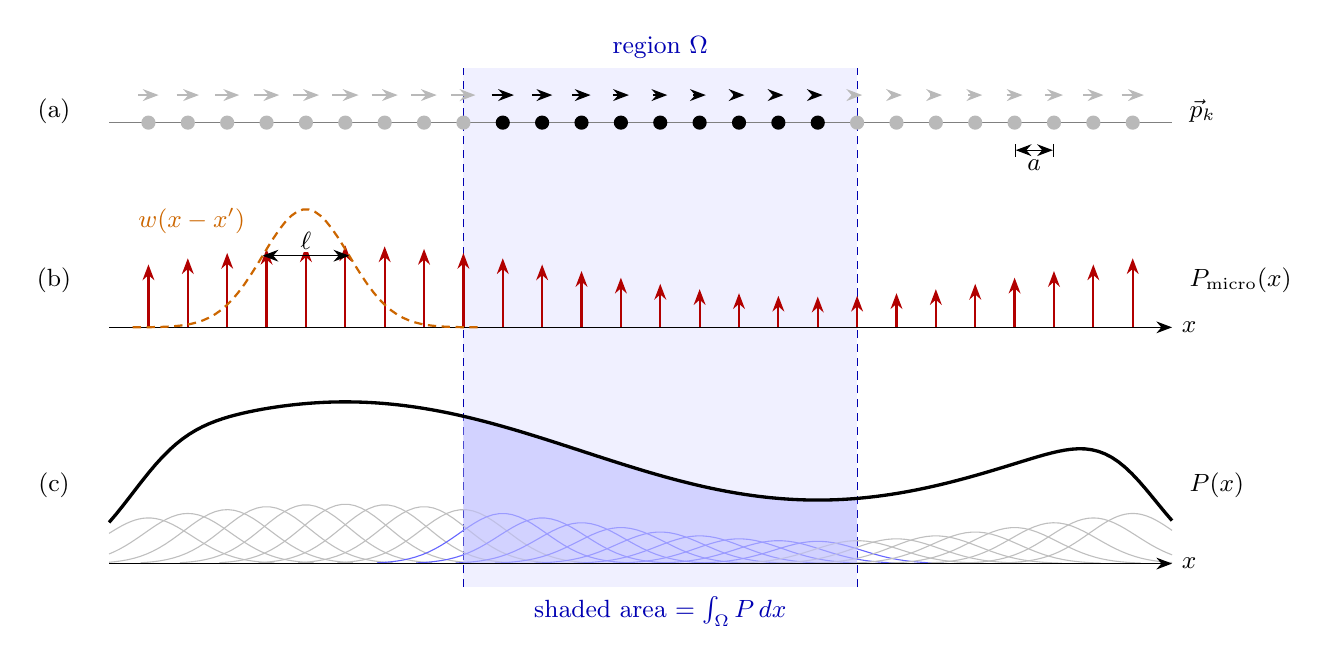
\begin{tikzpicture}[
  font=\small,
  >={Stealth[length=2mm]},
  declare function={
    spacing = 0.5;                                % interatomic distance a (cm)
    sig     = 0.55;                               % half-width of w (cm); width l ~ 2*sig
    pscale  = 1.3;                                % vertical plot scale of P(x)
    dip(\x) = 0.55 + 0.25*sin(deg(2*pi*\x/12));   % slowly varying dipole size p_k
  }
]
  % ---------- region Omega (spans all panels) ----------
  \def\xa{4.5}  \def\xb{9.5}
  \fill[blue!6] (\xa,-0.3) rectangle (\xb,6.3);
  \draw[densely dashed, blue!70!black] (\xa,-0.3) -- (\xa,6.3) (\xb,-0.3) -- (\xb,6.3);
  \node[blue!70!black] at ({(\xa+\xb)/2},6.55) {region $\Omega$};

  % ---------- (a) chain of atoms with dipoles ----------
  \node at (-0.7,5.75) {(a)};
  \draw[gray] (0,5.6) -- (13.5,5.6);
  \foreach \k in {1,...,26}{
    \pgfmathsetmacro{\xk}{\k*spacing}
    \pgfmathsetmacro{\len}{0.42*dip(\xk)}
    \pgfmathtruncatemacro{\inside}{(\xk>\xa) && (\xk<\xb)}
    \ifnum\inside=1 \def\col{black}\else\def\col{gray!55}\fi
    \fill[\col] (\xk,5.6) circle (0.09);
    \draw[->, thick, \col] ({\xk-\len/2},5.95) -- ({\xk+\len/2},5.95);
  }
  \draw[|<->|] (11.5,5.25) -- (12.0,5.25) node[midway, below] {$a$};
  \node[anchor=west] at (13.6,5.75) {$\vec p_k$};

  % ---------- (b) microscopic density and one averaging window ----------
  \node at (-0.7,3.6) {(b)};
  \draw[->] (0,3.0) -- (13.5,3.0) node[right] {$x$};
  \foreach \k in {1,...,26}{
    \pgfmathsetmacro{\xk}{\k*spacing}
    \draw[->, thick, red!70!black] (\xk,3.0) -- (\xk,{3.0+1.3*dip(\xk)});
  }
  % averaging window w centred at x' = 2.5
  \draw[thick, densely dashed, orange!80!black, domain=0.3:4.7, samples=60]
    plot (\x, {3.0 + 1.5*exp(-((\x-2.5)^2)/(2*sig^2))});
  \draw[<->] ({2.5-sig},{3.0+1.5*exp(-0.5)}) -- ({2.5+sig},{3.0+1.5*exp(-0.5)})
    node[midway, above=1pt, fill=white, inner sep=1pt] {$\ell$};
  \node[orange!80!black, anchor=east] at (1.85,4.35) {$w(x-x')$};
  \node[anchor=west] at (13.6,3.6) {$P_{\text{micro}}(x)$};

  % ---------- (c) smooth polarization ----------
  \node at (-0.7,1.0) {(c)};
  % build P(x) = sum_k p_k w(x - x_k) as one pgfmath expression
  \def\Psum{0}
  \foreach \k in {1,...,26}{
    \xdef\Psum{\unexpanded\expandafter{\Psum} + dip(\k*spacing)*exp(-((\noexpand\x-\k*spacing)^2)/(2*sig^2))}
  }
  \def\Pnorm{pscale/(sig*sqrt(2*pi))}   % normalization of w times the plot scale
  % individual contributions p_k w(x - x_k)
  \foreach \k in {1,...,26}{
    \pgfmathsetmacro{\xk}{\k*spacing}
    \pgfmathtruncatemacro{\inside}{(\xk>\xa) && (\xk<\xb)}
    \ifnum\inside=1 \def\col{blue!60}\else\def\col{gray!50}\fi
    \draw[\col, thin, domain={max(0,\xk-1.6)}:{min(13.5,\xk+1.6)}, samples=40]
      plot (\x, {\Pnorm*dip(\xk)*exp(-((\x-\xk)^2)/(2*sig^2))});
  }
  % area under P(x) inside Omega
  \fill[blue!25, opacity=0.6, domain=\xa:\xb, samples=60]
    (\xa,0) -- plot (\x, {\Pnorm*(\Psum)}) -- (\xb,0) -- cycle;
  \draw[very thick, domain=0:13.5, samples=160] plot (\x, {\Pnorm*(\Psum)});
  \draw[->] (0,0) -- (13.5,0) node[right] {$x$};
  \node[anchor=west] at (13.6,1.0) {$P(x)$};
  \node[blue!70!black, anchor=north] at ({(\xa+\xb)/2},-0.3) {shaded area $=\int_\Omega P\,dx$};
\end{tikzpicture}
\caption{Averaging of a one-dimensional chain of dipoles. (a)~Discrete dipoles $\vec p_k$ with interatomic distance $a$; dipoles inside $\Omega$ in black. (b)~Microscopic dipole density as delta peaks, with one averaging window $w$ of width $\ell \gg a$. (c)~Contributions $p_k\,w(x-x_k)$ of single dipoles (thin curves) and their sum, the smooth polarization $P(x)$ (thick curve). Dipoles far outside $\Omega$ (gray) do not contribute to the shaded area, and dipoles within $\ell$ of the boundary contribute partially.}
\label{fig:averaging}
\end{figure}

\paragraph{Limitation of the averaging picture in periodic crystals.}
The averaging assumes that the charge can be grouped into localized dipoles $\vec p_k$. In a periodic crystal, the electron density is continuous, so the dipole moment of a unit cell depends on how the cell is chosen. Different choices give bulk polarizations that differ by integer multiples of a \textcolor{blue}{polarization quantum}, which is proportional to a lattice vector divided by the cell volume. Only changes in $\vec P$, for example under strain or atomic displacement, are physical. The modern theory of polarization computes these changes from the Berry phase of the Bloch wave functions (King-Smith and Vanderbilt, 1993; Resta, 1994).

\paragraph{Electric field of a single dipole.}
The field of a volume of dipoles is built from the field of a single dipole. For a point dipole $\vec p$ at the origin, the dipole term of the multipole expansion gives the potential
\begin{equation*}
    \phi(\vec R) = \frac{\hat R\cdot\vec p}{R^2} = \frac{\vec p\cdot\vec R}{R^3}.
\end{equation*}
The electric field is the negative gradient of the potential, $\vec E = -\vec\nabla\phi$. With $\vec\nabla(\vec p\cdot\vec R) = \vec p$ and $\vec\nabla R^{-3} = -3\vec R/R^5$,
\begin{equation*}
    \vec E(\vec R) = -\frac{\vec p}{R^3} + \frac{3(\vec p\cdot\vec R)\,\vec R}{R^5}.
\end{equation*}
The field of a point dipole is therefore
\begin{equation}
    \boxed{
    \vec E(\vec R) = \frac{3(\vec p\cdot\hat R)\,\hat R - \vec p}{R^3}.
    }
\end{equation}

\paragraph{Potential of a volume of dipoles.}
Because $\vec P$ is a smooth density, the volume element $d^3r$ at the source point $\vec r$ carries the dipole moment $\vec P(\vec r)\,d^3r$. A dipole at $\vec r$ instead of the origin has the potential $\vec p\cdot(\vec R - \vec r)/|\vec R - \vec r|^3$. Summing the contributions of all volume elements of a material occupying $\Omega$ gives
\begin{equation*}
    \phi(\vec R) = \int_\Omega \frac{\vec P(\vec r)\cdot(\vec R - \vec r)}{|\vec R - \vec r|^3}\,d^3r.
\end{equation*}
\textcolor{red}{From now on, $\vec\nabla_{\vec r}$ denotes the gradient with respect to the source point $\vec r$, whereas $\vec\nabla$ without a subscript still acts on the field point $\vec R$.} The integrand simplifies with the identity
\begin{equation*}
    \vec\nabla_{\vec r}\,\frac{1}{|\vec R - \vec r|} = \frac{\vec R - \vec r}{|\vec R - \vec r|^3},
\end{equation*}
so that
\begin{equation*}
    \phi(\vec R) = \int_\Omega \vec P\cdot\vec\nabla_{\vec r}\,\frac{1}{|\vec R - \vec r|}\,d^3r.
\end{equation*}

\paragraph{Bound charges as the sources of the polarization potential.}
The product rule $\vec\nabla_{\vec r}\cdot(f\vec P) = f\,\vec\nabla_{\vec r}\cdot\vec P + \vec P\cdot\vec\nabla_{\vec r} f$ with $f = 1/|\vec R - \vec r|$ splits the integrand into two parts,
\begin{equation*}
    \phi(\vec R) = \int_\Omega \vec\nabla_{\vec r}\cdot\left(\frac{\vec P}{|\vec R - \vec r|}\right) d^3r
    - \int_\Omega \frac{\vec\nabla_{\vec r}\cdot\vec P}{|\vec R - \vec r|}\,d^3r.
\end{equation*}
The divergence theorem turns the first integral into an integral over the boundary $\partial\Omega$, with outward unit normal $\hat n$ and surface element $dS$. The potential of the polarized material is therefore
\begin{equation}
    \boxed{
    \begin{gathered}
    \phi(\vec R) = \oint_{\partial\Omega} \frac{\sigma_b(\vec r)}{|\vec R - \vec r|}\,dS
    + \int_\Omega \frac{\rho_b(\vec r)}{|\vec R - \vec r|}\,d^3r,\\[4pt]
    \sigma_b = \vec P\cdot\hat n, \qquad \rho_b = -\vec\nabla_{\vec r}\cdot\vec P,
    \end{gathered}
    }
\end{equation}
where $\sigma_b$ is the \textcolor{blue}{bound surface charge density} and $\rho_b$ is the \textcolor{blue}{bound volume charge density}. A polarized material thus produces the same potential as these two charge distributions. In particular, a uniform polarization has $\rho_b = 0$ and produces only a surface charge. Figure~\ref{fig:boundcharge} shows the origin of both bound charges in a chain of dipoles.

\begin{figure}[htbp]
\centering
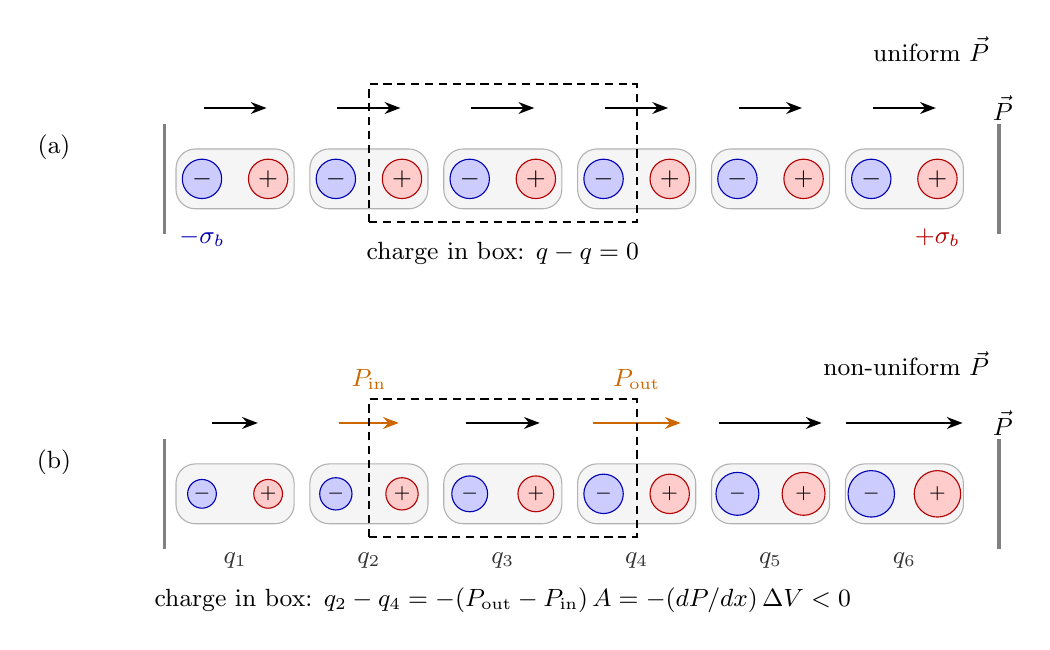
\begin{tikzpicture}[
  font=\small,
  >={Stealth[length=2mm]},
  negcharge/.style={circle, draw=blue!70!black, fill=blue!20, inner sep=0pt},
  poscharge/.style={circle, draw=red!70!black,  fill=red!20,  inner sep=0pt},
  mol/.style={rounded corners=7pt, draw=gray!60, fill=gray!8},
  box/.style={thick, densely dashed},
]
  % ============ (a) uniform polarization ============
  \begin{scope}[yshift=4.0cm]
    \node at (-0.6,0.4) {(a)};
    \node[anchor=east] at (11.4,1.65) {uniform $\vec P$};
    \foreach \k in {1,...,6}{
      \pgfmathsetmacro{\c}{1.7*\k}
      \draw[mol] ({\c-0.75},-0.38) rectangle ({\c+0.75},0.38);
      \node[negcharge, minimum size=5mm] at ({\c-0.42},0) {$-$};
      \node[poscharge, minimum size=5mm] at ({\c+0.42},0) {$+$};
      \draw[->, thick] ({\c-0.4},0.9) -- ({\c+0.4},0.9);
    }
    \node[anchor=west] at (11.2,0.9) {$\vec P$};
    \draw[very thick, gray] (0.8,-0.7) -- (0.8,0.7) (11.4,-0.7) -- (11.4,0.7);
    \node[blue!70!black] at (1.28,-0.75) {$-\sigma_b$};
    \node[red!70!black]  at (10.62,-0.75) {$+\sigma_b$};
    % box from the centre of dipole 2 to the centre of dipole 4
    \draw[box] (3.4,-0.55) rectangle (6.8,1.2);
    \node at (5.1,-0.95) {charge in box: $q - q = 0$};
  \end{scope}

  % ============ (b) non-uniform polarization ============
  \node at (-0.6,0.4) {(b)};
  \node[anchor=east] at (11.4,1.65) {non-uniform $\vec P$};
  \foreach \k in {1,...,6}{
    \pgfmathsetmacro{\c}{1.7*\k}
    \pgfmathsetmacro{\s}{3.2+0.45*\k}      % circle size grows with q_k
    \pgfmathsetmacro{\L}{0.2+0.09*\k}      % arrow half-length grows with P
    \draw[mol] ({\c-0.75},-0.38) rectangle ({\c+0.75},0.38);
    \node[negcharge, minimum size=\s mm] at ({\c-0.42},0) {\scriptsize$-$};
    \node[poscharge, minimum size=\s mm] at ({\c+0.42},0) {\scriptsize$+$};
    \ifnum\k=2 \def\col{orange!80!black}\else\ifnum\k=4 \def\col{orange!80!black}\else\def\col{black}\fi\fi
    \draw[->, thick, \col] ({\c-\L},0.9) -- ({\c+\L},0.9);
    \node[gray!40!black] at (\c,-0.85) {$q_{\k}$};
  }
  \node[anchor=west] at (11.2,0.9) {$\vec P$};
  \draw[very thick, gray] (0.8,-0.7) -- (0.8,0.7) (11.4,-0.7) -- (11.4,0.7);
  % box from the centre of dipole 2 to the centre of dipole 4
  \draw[box] (3.4,-0.55) rectangle (6.8,1.2);
  \node[orange!80!black, anchor=south] at (3.4,1.2) {$P_{\text{in}}$};
  \node[orange!80!black, anchor=south] at (6.8,1.2) {$P_{\text{out}}$};
  \node at (5.1,-1.35) {charge in box: $q_2 - q_4 = -(P_{\text{out}}-P_{\text{in}})\,A = -(dP/dx)\,\Delta V < 0$};
\end{tikzpicture}
\caption{Bound charges of a chain of dipoles between two surfaces. (a)~Uniform polarization: the charges of neighboring dipoles cancel inside the box, and only the surfaces carry the uncompensated charges $\pm\sigma_b$. (b)~Polarization increasing to the right: the box holds $+q_2$ and $-q_4$ with $q_4 > q_2$, so it carries the net charge $-(dP/dx)\,\Delta V$. Here $A$ is the cross-sectional area and $\Delta V$ the volume of the box.}
\label{fig:boundcharge}
\end{figure}

\section{Dielectric Sphere inside a Dielectric Medium}

\subsection{Gauss's Law in a Polarizable Material}

\paragraph{Electric displacement as the field of the free charges.}
Gauss's law counts both the \textcolor{blue}{free charge} $\rho_f$ and the bound charge $\rho_b$,
\begin{equation*}
    \vec\nabla\cdot\vec E = 4\pi(\rho_f + \rho_b), \qquad \rho_b = -\vec\nabla\cdot\vec P.
\end{equation*}
The bound charge is unknown until $\vec E$ is known. Moving it to the left side defines the \textcolor{blue}{electric displacement} $\vec D$,
\begin{equation}
    \boxed{
    \vec D = \vec E + 4\pi\vec P, \qquad \vec\nabla\cdot\vec D = 4\pi\rho_f.
    }
\end{equation}
This is only a change of variables; a relation between $\vec P$ and $\vec E$ is still needed.

\paragraph{Linear response and the dielectric tensor.}
For a weak field, the polarization is expanded to first order about $\vec E = 0$,
\begin{equation*}
    P_\alpha(\vec E) = P_\alpha(0) + \sum_\beta \chi_{\alpha\beta}E_\beta + \mathcal{O}(E^2),
    \qquad
    \chi_{\alpha\beta} = \left.\frac{\partial P_\alpha}{\partial E_\beta}\right|_{\vec E = 0}.
\end{equation*}
With $P_\alpha(0) = 0$ and without the $\mathcal{O}(E^2)$ terms,
\begin{equation}
    \boxed{
    P_\alpha = \sum_\beta \chi_{\alpha\beta}E_\beta, \qquad
    D_\alpha = \sum_\beta \varepsilon_{\alpha\beta}E_\beta, \qquad
    \varepsilon_{\alpha\beta} = \delta_{\alpha\beta} + 4\pi\chi_{\alpha\beta},
    }
\end{equation}
where $\chi_{\alpha\beta}$ is the \textcolor{blue}{susceptibility tensor} and $\varepsilon_{\alpha\beta}$ is the \textcolor{blue}{dielectric tensor}. Here $\vec E$ is the macroscopic field at the same point, not the external field.

\paragraph{Isotropic materials and the dielectric constant.}
An \textcolor{blue}{isotropic} material responds equally in every direction, $\chi_{\alpha\beta} = \chi\,\delta_{\alpha\beta}$, so that
\begin{equation}
    \boxed{
    \vec P = \chi\,\vec E, \qquad \vec D = \varepsilon\,\vec E, \qquad \varepsilon = 1 + 4\pi\chi,
    }
\end{equation}
where $\chi$ is the \textcolor{blue}{electric susceptibility} and $\varepsilon$ is the \textcolor{blue}{dielectric constant}.

\paragraph{Limits of the linear model.}
Each assumption above fails in some materials. A ferroelectric carries a spontaneous polarization, $\vec P(0) = \vec P_s \neq 0$. A strong field, as in nonlinear optics, makes the second-order term significant,
\begin{equation*}
    P_\alpha = \sum_\beta \chi_{\alpha\beta}E_\beta + \sum_{\beta,\gamma}\chi^{(2)}_{\alpha\beta\gamma}E_\beta E_\gamma + \mathcal{O}(E^3).
\end{equation*}
A time-dependent field gives a frequency-dependent response, $\vec P(\omega) = \chi(\omega)\,\vec E(\omega)$; for example, metals at optical frequencies have $\varepsilon(\omega) < 0$. This note treats static, weak fields in linear isotropic media only.

\subsection{Boundary Conditions between Two Dielectric Media}

\paragraph{Laplace's equation inside each medium.}
Consider two linear isotropic media, labeled 1 and 2, with constant dielectric constants $\varepsilon_1$ and $\varepsilon_2$ and $\rho_f = 0$. With $\vec D = -\varepsilon\vec\nabla\phi$,
\begin{equation*}
    \vec\nabla\cdot\vec D = -\varepsilon\,\nabla^2\phi = 0,
\end{equation*}
so the potential satisfies Laplace's equation in both media,
\begin{equation}
    \boxed{
    \nabla^2\phi_1 = 0, \qquad \nabla^2\phi_2 = 0.
    }
\end{equation}

\paragraph{Normal component from the divergence theorem.}
Let $\hat n$ be the unit normal to the interface, pointing from medium 1 into medium 2, with $\partial/\partial n = \hat n\cdot\vec\nabla$ and $D_n = \vec D\cdot\hat n$. A pillbox of face area $\Delta A$ and height $h$ straddles the interface. The divergence theorem gives
\begin{equation*}
    \oint_{\text{pillbox}} \vec D\cdot d\vec A = \int_{\text{pillbox}} \vec\nabla\cdot\vec D\;d^3r = 4\pi Q_f = 0.
\end{equation*}
As $h \to 0$, the side wall drops out and only the two faces remain,
\begin{equation*}
    \left(D_{2,n} - D_{1,n}\right)\Delta A = 0
    \quad\Rightarrow\quad
    \varepsilon_1 E_{1,n} = \varepsilon_2 E_{2,n}.
\end{equation*}
With $E_n = -\partial\phi/\partial n$,
\begin{equation}
    \boxed{
    \varepsilon_1\frac{\partial\phi_1}{\partial n} = \varepsilon_2\frac{\partial\phi_2}{\partial n}.
    }
\end{equation}
The same pillbox applied to $\vec E$ encloses the bound surface charge, $E_{2,n} - E_{1,n} = 4\pi\sigma_b$, so $E_n$ itself jumps across the interface.

\paragraph{Tangential component from Stokes' theorem.}
In electrostatics, $\partial\vec B/\partial t = 0$, so Faraday's law gives $\vec\nabla\times\vec E = 0$. Let $C$ be a rectangular loop with two sides of length $\Delta l$ along a tangent $\hat t$ of the interface, one in each medium, and two sides of height $h$ crossing it. Stokes' theorem gives
\begin{equation*}
    \oint_C \vec E\cdot d\vec l = \int_S \left(\vec\nabla\times\vec E\right)\cdot d\vec S = 0,
\end{equation*}
where $S$ is the surface bounded by $C$. As $h \to 0$, only the two long sides remain,
\begin{equation*}
    \left(E_{2,t} - E_{1,t}\right)\Delta l = 0
    \quad\Rightarrow\quad
    E_{1,t} = E_{2,t}.
\end{equation*}
The same theorem forbids closed field lines, because $\vec E\cdot d\vec l > 0$ along a field line and $\oint\vec E\cdot d\vec l$ would be positive. Across the interface, the potential difference over the height $h$ vanishes for a finite field,
\begin{equation*}
    \phi_2 - \phi_1 = -\int_0^h \vec E\cdot\hat n\;dl \;\longrightarrow\; 0 \qquad (h \to 0),
\end{equation*}
which gives
\begin{equation}
    \boxed{
    \phi_1 = \phi_2 \quad \text{on the interface}.
    }
\end{equation}
Since $E_t = -\hat t\cdot\vec\nabla\phi$ and $\phi_1 = \phi_2$ holds all along the interface, this condition contains $E_{1,t} = E_{2,t}$.

\end{document}